\documentclass[]{beamer}
\usepackage{mathptmx}
\usepackage{amsmath, amsfonts, epsfig, xspace}
\usepackage{algorithm,algorithmic}
\usepackage{pstricks,pst-node}
\usepackage{multimedia}
\usepackage[normal,tight,center]{subfigure}
\setlength{\subfigcapskip}{-.5em}
\usepackage{beamerthemesplit}
\usepackage{graphicx}
\usepackage[framemethod=tikz]{mdframed}
\usetheme{lankton-keynote}
\setbeamerfont{frametitle}{size=\medium}
\setbeamerfont{block title}{size=\scriptsize}
\setbeamertemplate{caption}{\raggedright\insertcaption\par}

\usefonttheme{professionalfonts}
\usepackage[T1]{fontenc}
\usepackage{libertine}
\renewcommand{\ttdefault}{cmtt}

\title{X-ray Reverberation in~AGN}
\author[Stephen Hancock]{Stephen Hancock \\Supervised by Andy Young}

\begin{document}
\begin{frame}
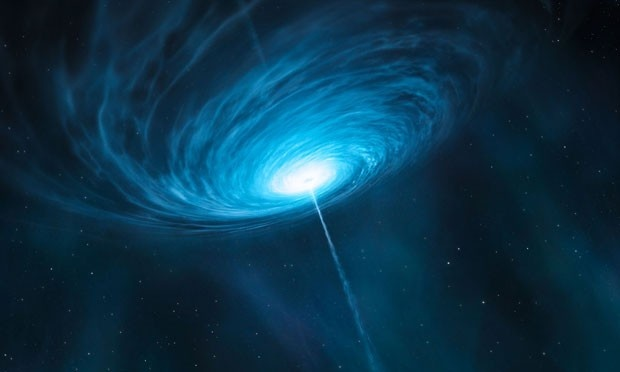
\includegraphics[width=\textwidth,height=.45\textheight]{bh2.jpg}
\titlepage
\end{frame}

\begin{frame}
\frametitle{Overview}
\centering
X-ray observations of Active Galactic Nuclei (AGN) can be used to study their dynamic environment via reflected radiation from the innermost regions of the accretion disk
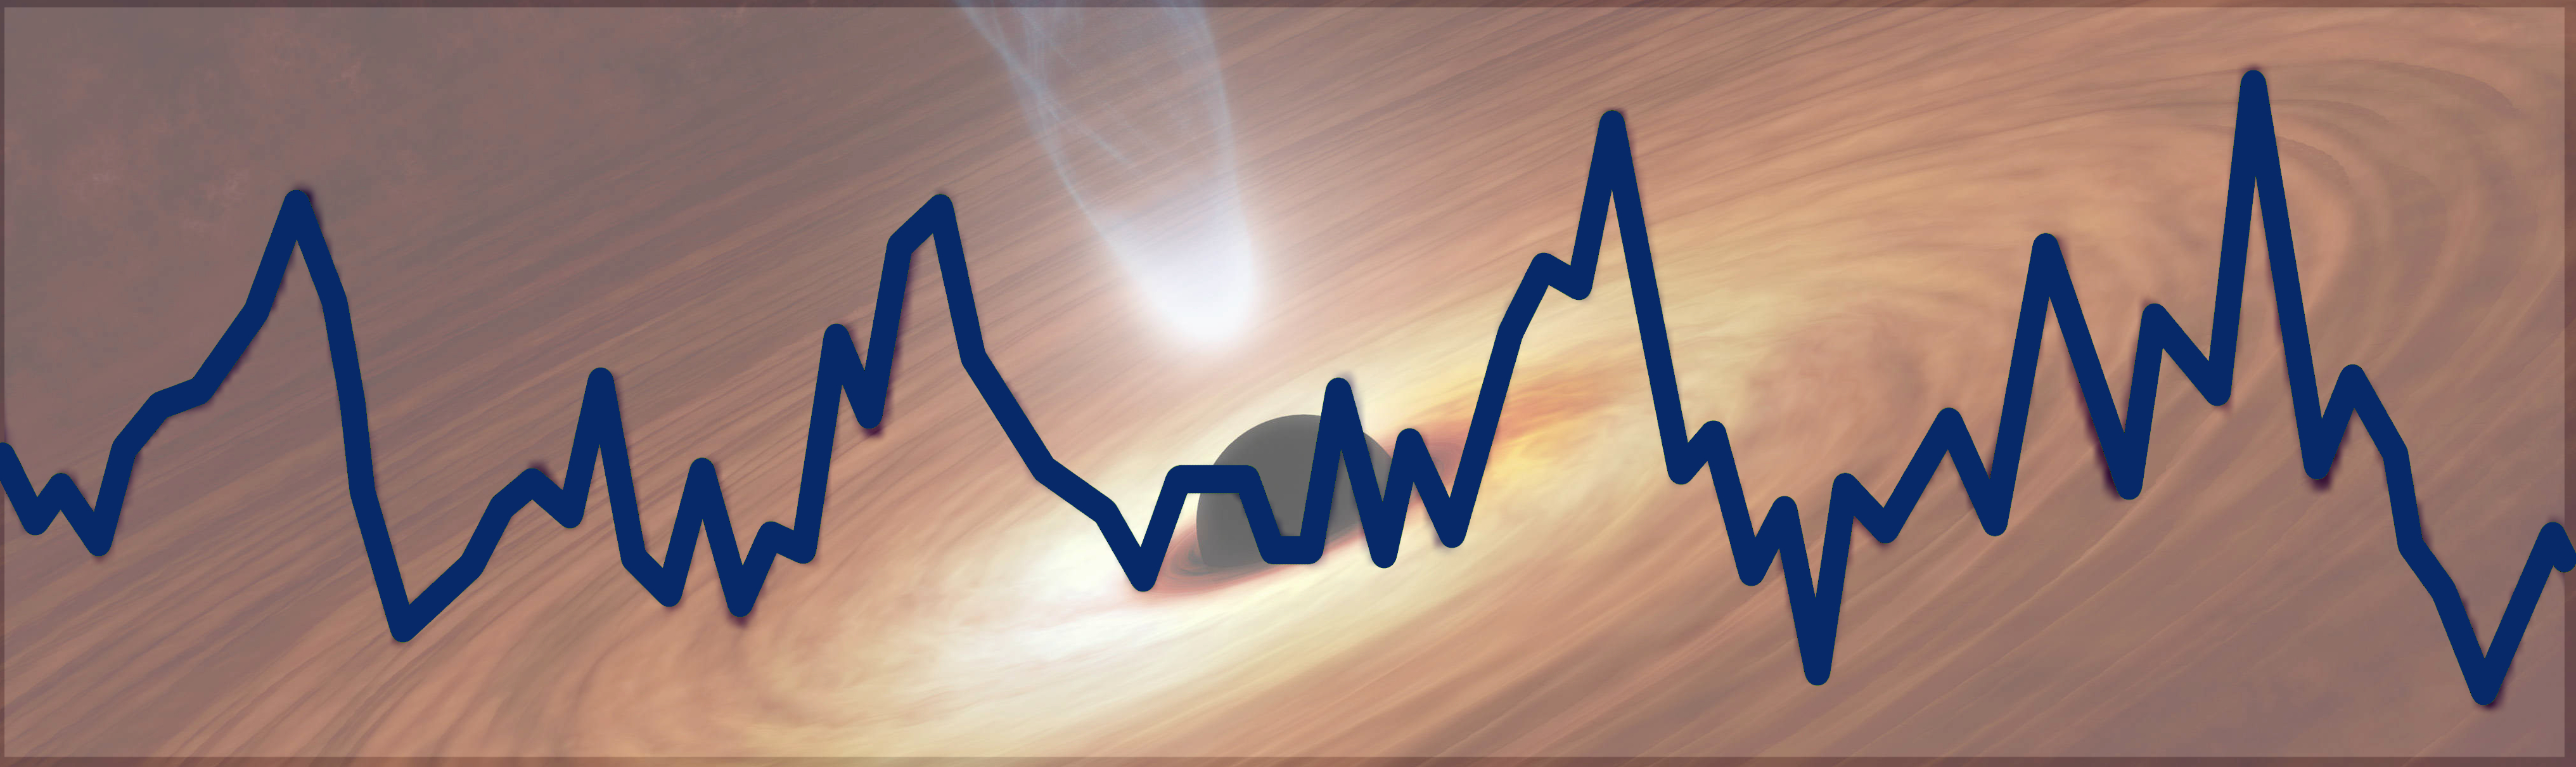
\includegraphics[width=\textwidth,height=.45\textheight]{agn2.jpg}

\end{frame}

\begin{frame}
[t]{X-ray reverberation in AGN}
    \begin{columns}%[T,onlytextwidth]
        \begin{column}{.45\textwidth}
            \begin{minipage}{\textwidth}
                \begin{figure}
                \colorbox{white}{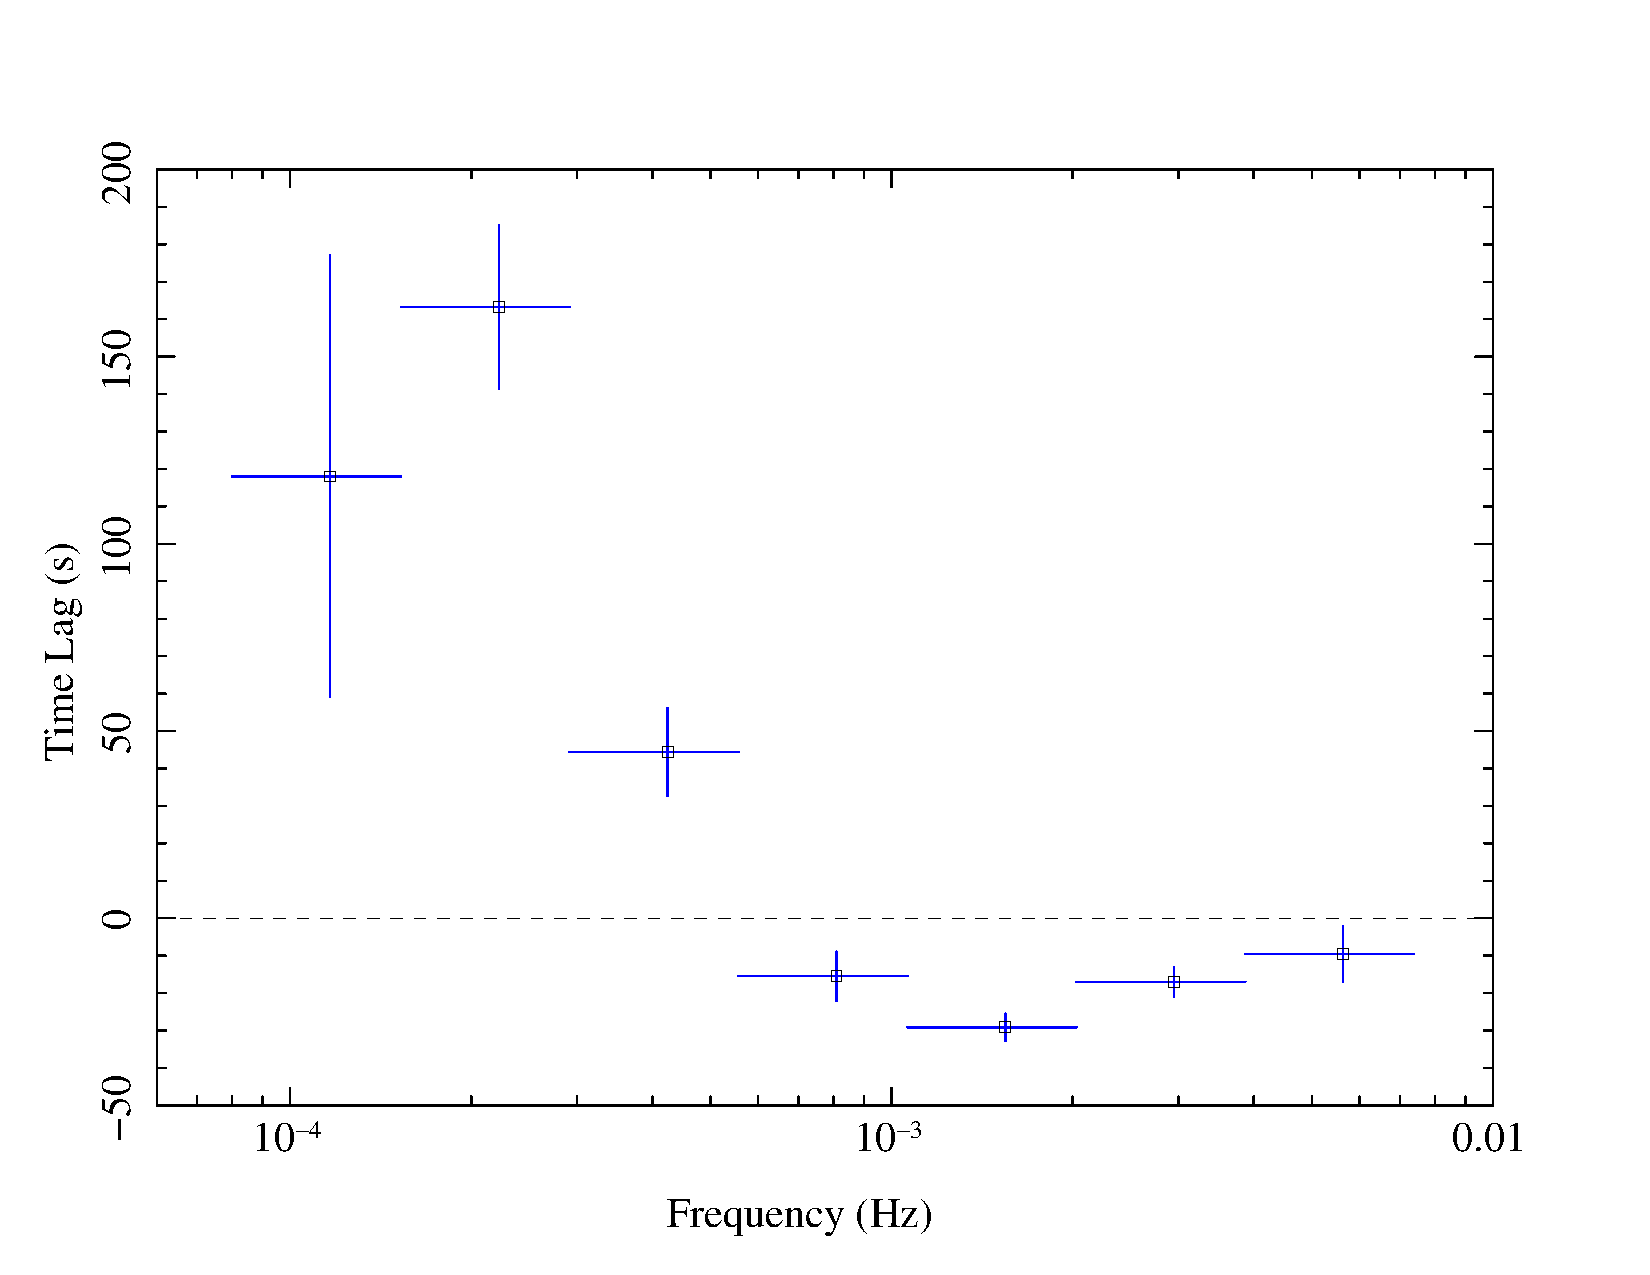
\includegraphics[scale=0.16]{1H0707-495_lagfreq_fullycomb.pdf}}\\~\\
                \end{figure}
                %\footnotetext{Lag-frequency}
            \end{minipage}  
            \begin{onlyenv}<1>
                \begin{minipage}{\textwidth}
                    \begin{figure}\centering
                    \colorbox{white}{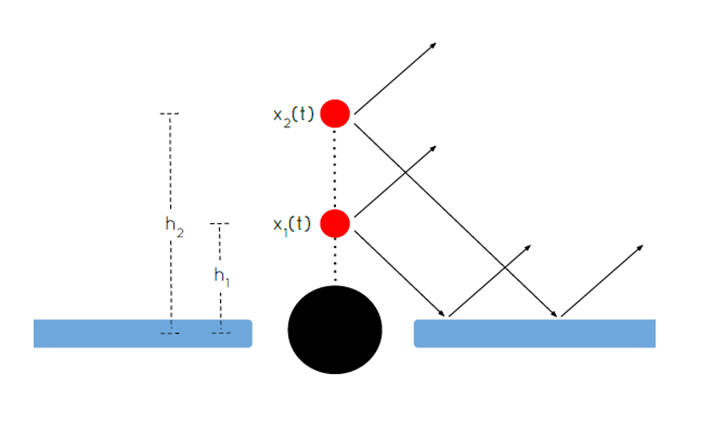
\includegraphics[width=4.5cm]{2bm.png}}
                    \end{figure}
                %\footnotetext{Extended Corona}
                \end{minipage}
            \end{onlyenv}
        \end{column}
        \begin{column}{.4\textwidth}
            \begin{onlyenv}
                \begin{minipage}{\textwidth}
                    \begin{figure}
                        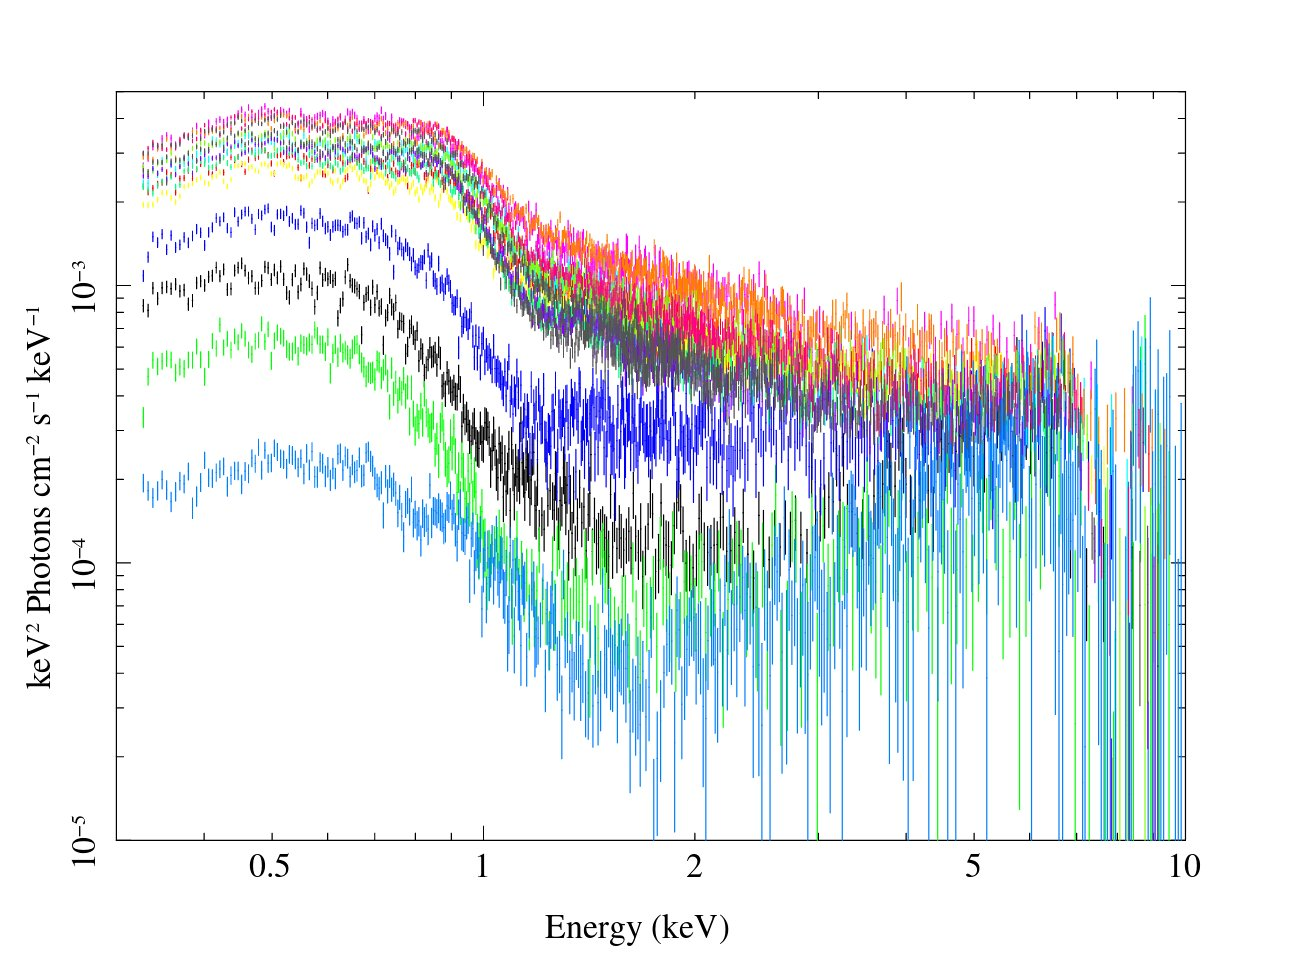
\includegraphics[scale=0.14]{1H0707-495_Unfolded_Spectra.jpeg}\\~\\
                    \end{figure}
                    %\footnotetext{Spectrum}
                \end{minipage}
            \end{onlyenv}
            \begin{minipage}{\textwidth}
                    \begin{figure}
                        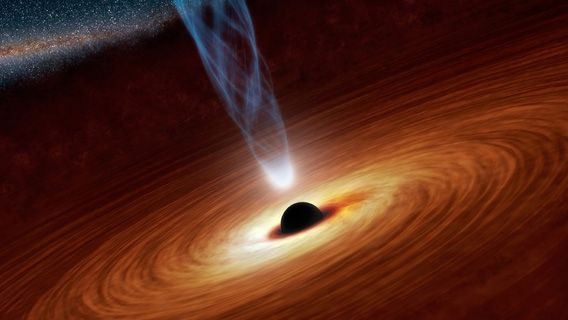
\includegraphics[width=5.0cm]{bh1.jpg}
                    \end{figure}
                \end{minipage}
        \end{column}
    \end{columns}
\end{frame}


\begin{frame}
\frametitle{Reverberation Lags: Aims}
\setbeamercovered{transparent}
 \noindent\begin{minipage}[t]{.45\textwidth}
  Explore Lag-frequency and spectra of 20 AGN:
  \begin{itemize}
  \item Calculate time lags for all observations
  \item Explore spectral properties
  \item Reflection modelling 
  \item Absorption modelling
  \end{itemize}
 \end{minipage}\hspace{.5cm}  % <--- space
\pause
 \begin{minipage}[t]{.45\textwidth}
   Develop the Extended Corona Model:
   \begin{itemize}
   \item Build on BC4
   \item Apply model to AGN lag-frequency models
   \item Source heights $H_1$ and $H_2$ ~ 2 - 20 $r_g$
   \item Explore results
   \item Automate Model
   \item Publicly available
 \end{itemize}
 \end{minipage}
\end{frame}

\begin{frame}
\frametitle{The broad iron line}
\begin{columns}
\column{0.5\textwidth}
{
    \begin{figure}
    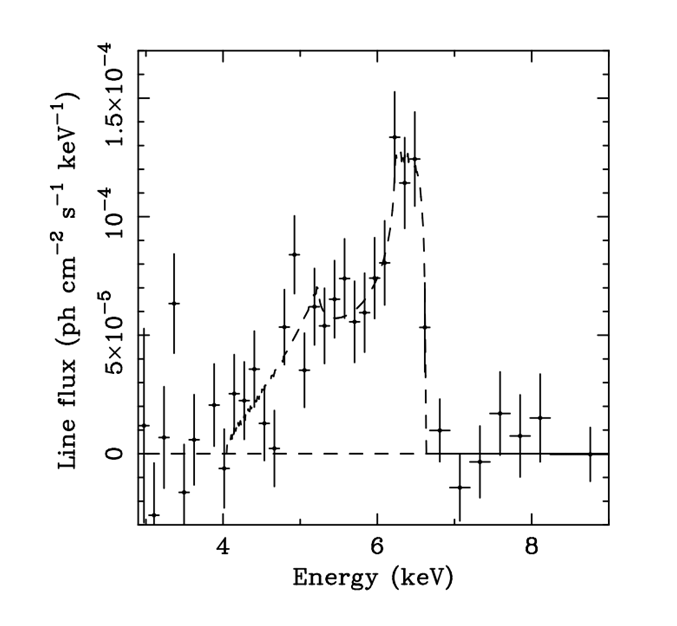
\includegraphics[width=\textwidth,height=.5\textheight]{broadKline.png}\\
    \caption{Fe line in MCG--6-30-15 (Tanaka et al. 1995)}
    \end{figure}
}
\column{0.5\textwidth}
\begin{itemize}
    \item Illumination of the disc produces narrow Fe K$\alpha$ line at 6.4~keV in the rest frame
    \item ASCA observation of MCG--6-30-15 show the Fe line is broadened and skewed to lower energies
    \item Fe K$\alpha$ emission interpreted as originating from the inner regions of the disc close to a black hole
\end{itemize}
\end{columns}
\end{frame}

\begin{frame}
\frametitle{XMM-Newton - Key Features}
\begin{figure}
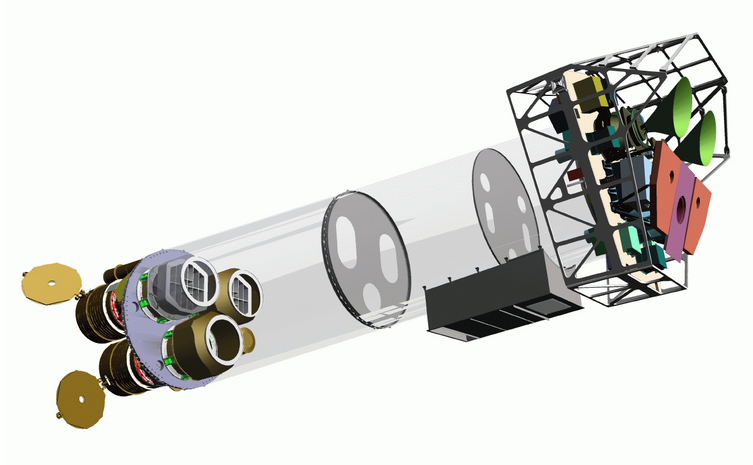
\includegraphics[scale=.25]{xmm-newton-glass.png} 
\end{figure}
\item 3 CCD European Photon Imaging Camera (EPIC) 
cameras for X-ray imaging, moderate resolution spectroscopy, and X-ray photometry; two different types of EPIC cameras are MOS and pn.
\item Reflection Grating Spectrometer (RGS) for high-resolution X-ray spectroscopy and spectro-photometry.
\item Optical Monitor (OM) for optical/UV imaging and grism spectroscopy. 
\end{frame}

\begin{frame}
\frametitle{XMM-Newton (since 1999)}
\begin{figure}
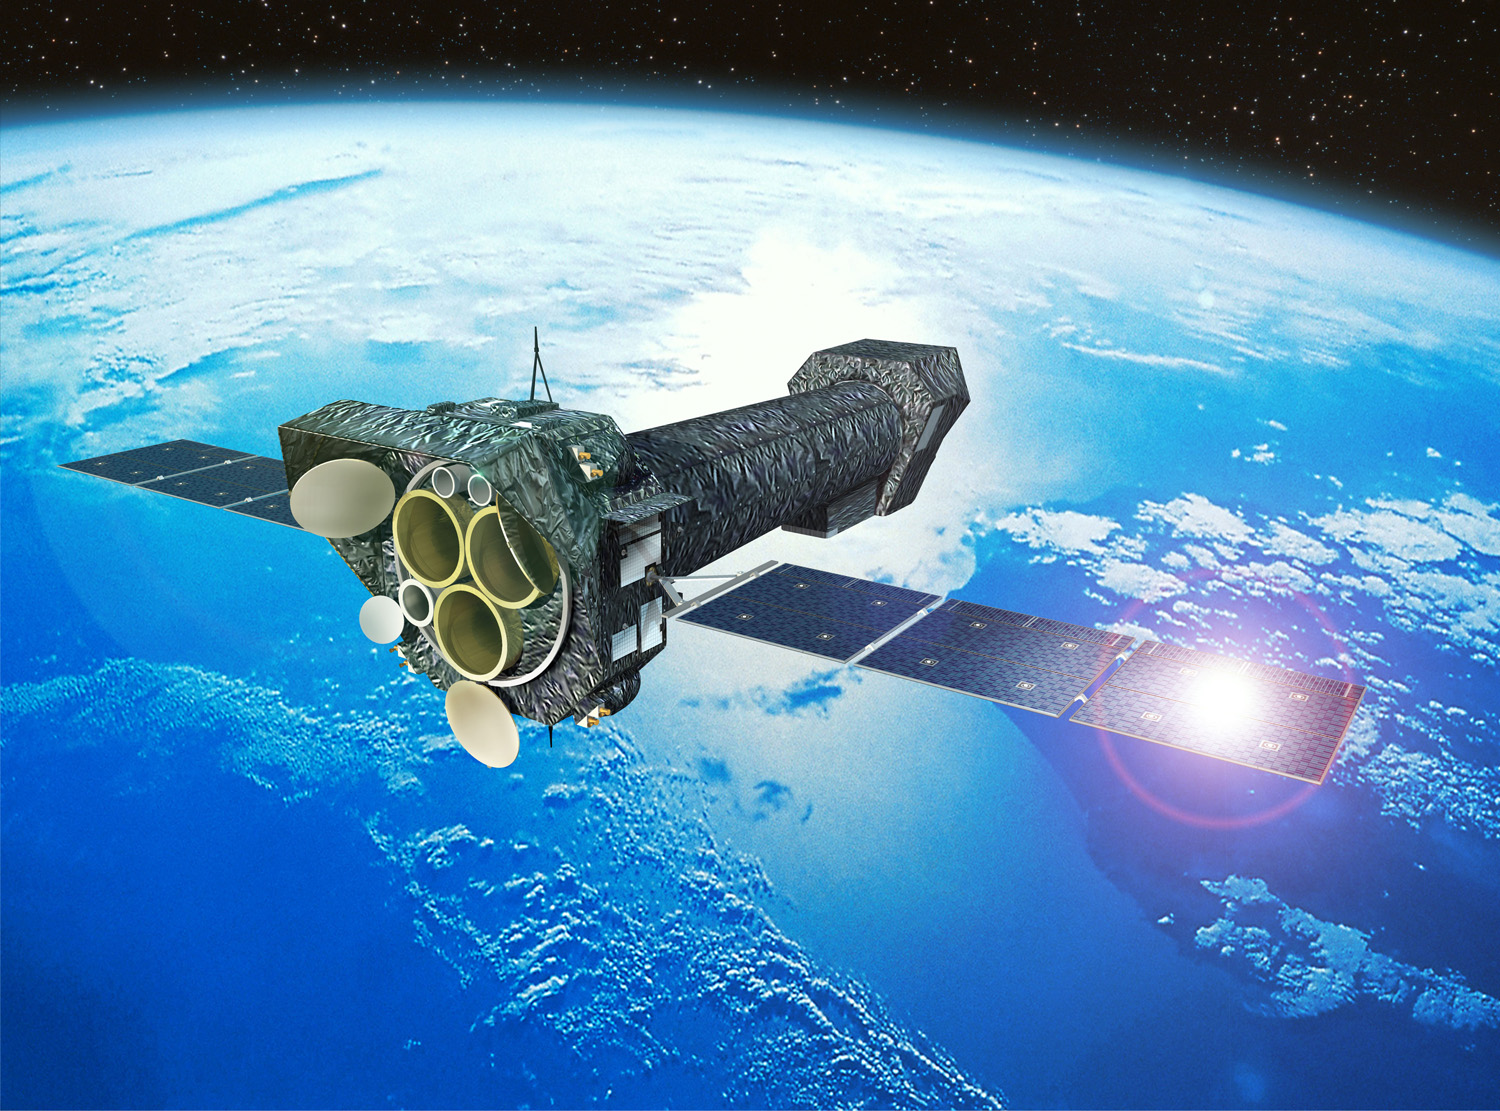
\includegraphics[scale=.30]{XMM-Newton_1500.jpg} 
\end{figure}
\item Spectral range of 0.15 - 12 keV
\item Large collective area over a 30 arcmin field of view in the 0.15--15 keV range
\item PSF is 6 arcsec FWHM
\item Capable of conducting long uninterrupted observations
\end{frame}

\begin{frame}
\frametitle{The problem}

\begin{itemize}
\item The Fe K$\alpha$ emission should vary in flux with the continuum \pause

\item However, the illuminating flux exhibits large amplitude variability while the red wing of the Fe K$\alpha$ line appears largely invariant \pause 

\item To address this problem Miniutti \& Fabian (2004) proposed a light bending model where light follows curved geodesics close to the black hole \pause

\item The reflection flux may be almost invariant while the observed continuum flux can show significant variability as the source changes height above the disc
\end{itemize}
\end{frame}

\begin{frame}
\frametitle{The Lamppost scenario} \centering 
{
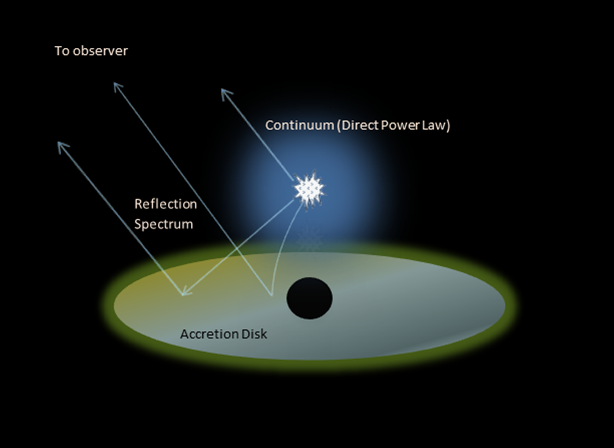
\includegraphics[scale=0.6]{lampost1.png}\\
}
\end{frame}

\begin{frame}
\centering
\large{The Lag-frequency}
\end{frame}


\
\begin{frame} <presentation:0>
\frametitle{ECM Parameters}
\begin{figure} \centering
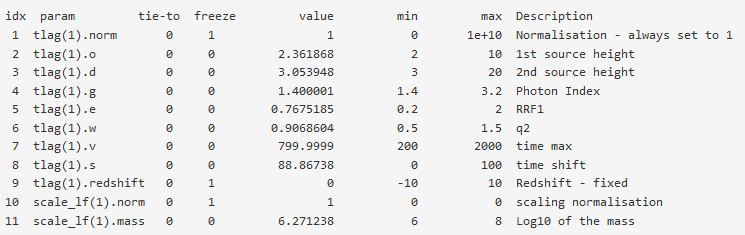
\includegraphics[scale=.55]{2bm_param.png}
\end{figure}
\begin{itemize}
{\footnotesize  
    \item RRF1 is the reflection fraction
    \item $q_2$ is the source response modelled using a cut-off powerlaw: $\Psi_i(t) \propto t^{-q_i} exp(-t/t_{max})$
    \item $t_{shift} $ is the time taken for fluctuations to propagate from $h_1$ to $h_2$
    \item $t_{max}$ is time difference between the beginning and end of the response
    }
\end{itemize}
\end{frame}


\begin{frame}{}
\centering
Methods 
\end{frame}

\begin{frame}{Methods: 1H0707-495 Example}
\centering
1H0707-495 was observed by XMM-Newton many times between 2000 - 2015\\
\vspace{0.5cm}
The following is an example of the analysis of a 40,600s observation taken in 2000
\end{frame}


\begin{frame}{Methods: 1H0707-495 Observation 2000}
%\centering
\begin{figure}
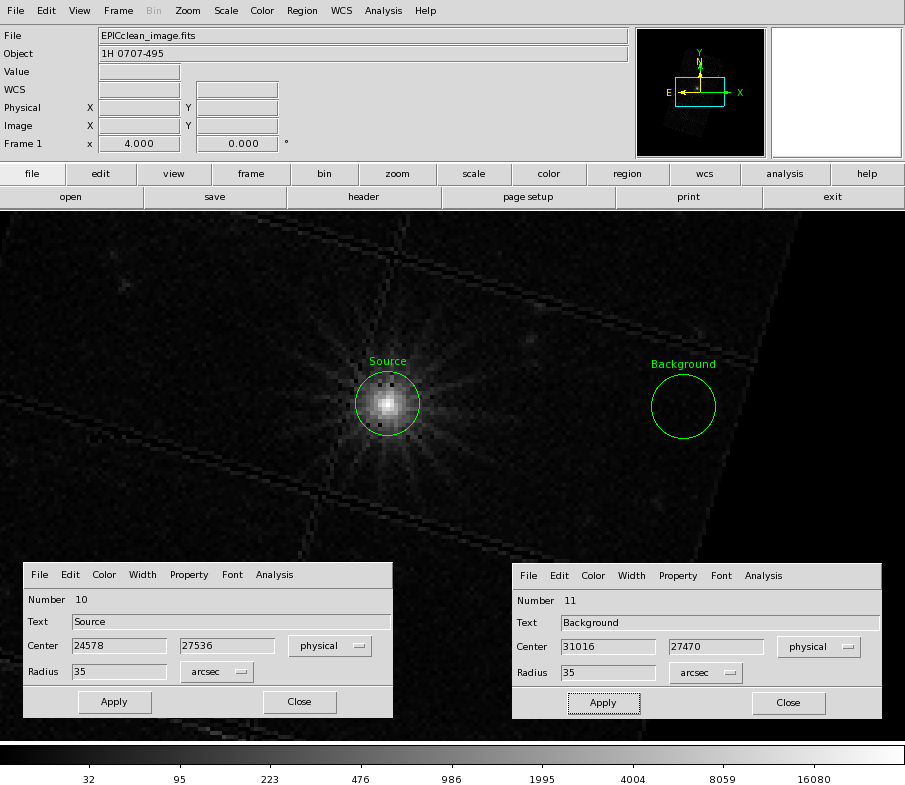
\includegraphics[scale=0.30]{1H0707-495_0506200501_SrcBkg_Regions}
\end{figure}
\end{frame}

\begin{frame}
\frametitle{The lag-frequency}
\begin{columns}
\column{0.5\textwidth}
\begin{figure}
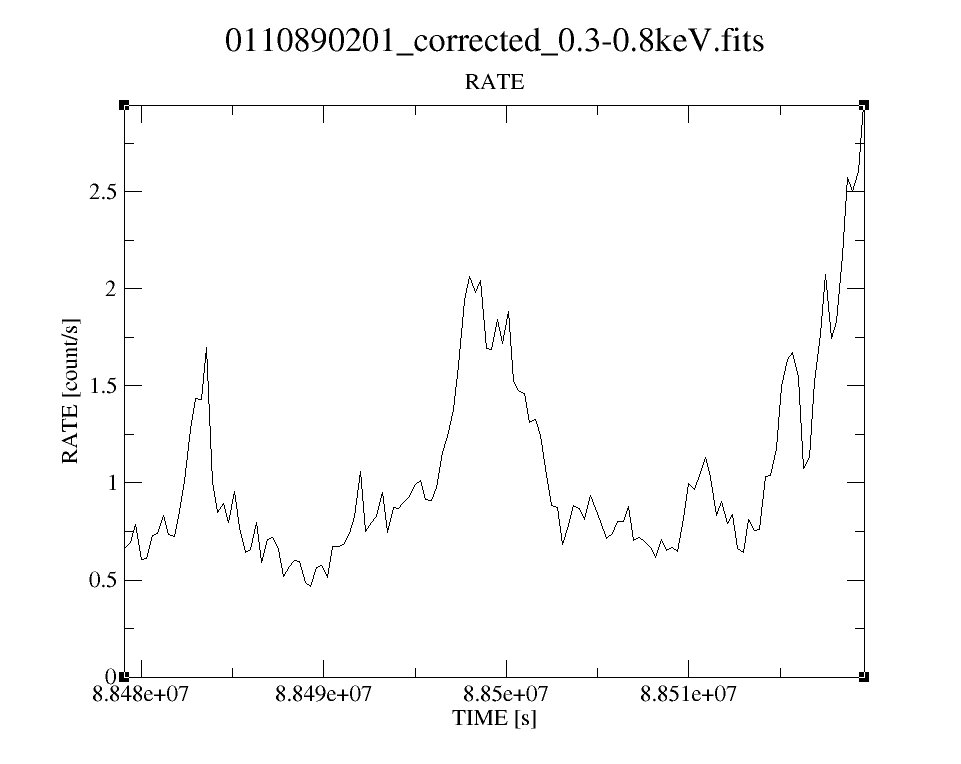
\includegraphics[scale=.182]{1H0707-495_0110890201_soft_lc} \\
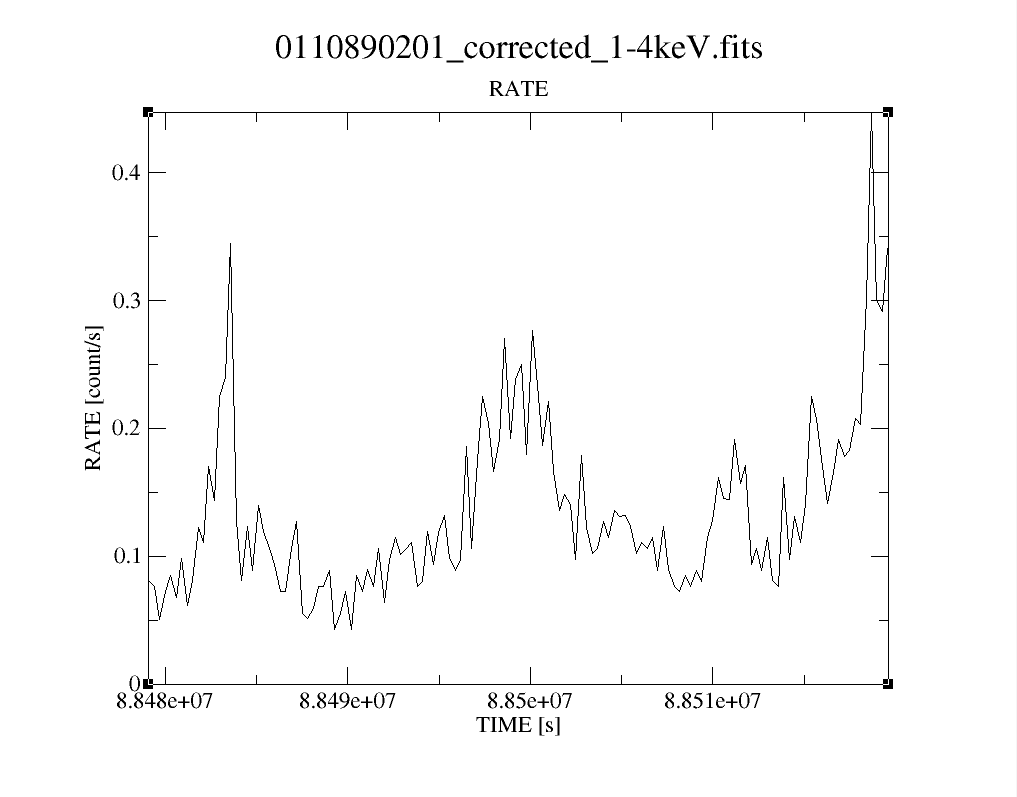
\includegraphics[scale=.174]{1H0707-495_0110890201_1-4keV_lc}
\end{figure}
\column{0.5\textwidth}
Using Fourier methods e.g; 
\begin{equation}
DFT_s(j)=\sum_{k=0}^{N}s(t_k) \exp\left(\frac{-2\pi ikj}{N}\right)\nonumber
\end{equation}
Time lags $\tau$ can calculated using the phase \\\vspace{0.2cm} $\tau(\nu_j)=\phi(\nu_j)/(2\pi\nu_j)$.
\end{columns}
\end{frame}

\begin{frame}
\frametitle{Methods in brief}
The time lags between the soft light curve $s(t)$ (0.3--0.8 keV) and the hard light curve $h(t)$ (1--4 keV) were computed using discrete Fourier transform (DFT) methods as outlined by Nowak+1999 and Uttley+2014.

\begin{equation}
DFT_s(j)=\sum_{k=0}^{N}s(t_k) \exp\left(\frac{-2\pi ikj}{N}\right)
\end{equation}
where $DFT_s (j)$ is the discrete Fourier transform at each Fourier frequency, $f_j=n/N$ for $j = 0, 1, 2, 3, ...N/2$ and $t_k$ is the $k$th value of the light curve. 
\end{frame}

\begin{frame}<presentation:0>
\frametitle{Methods in brief}
The Fourier cross spectrum between two curves $x(t)$ and $y(t)$ with DFTs $X_n$ and $Y_n$ was calculated using the real and imaginary components by:
\begin{equation}
C_X{}_Y{}_,{}_n= X_n^*Y_n
\end{equation}
and then multiplying by the complex conjugate of $X_n$ cancels out the phase $\psi_n$ and the cross spectrum giving the phase lag between the light curves was then derived by:
\begin{equation}
C_X{}_Y{}_,{}_n= A_X{}_,{}_n A_Y{}_,{}_n \exp [i\phi_n]
\end{equation}
\end{frame}

\begin{frame}<presentation:0>
\frametitle{Methods in brief}
The coherence $\gamma^2$ is a Fourier frequency dependent measure of the correlation between two light curves. It provides a fraction of the mean squared variability at a frequency of one light curve that can be predicted by the other. The coherence function $\gamma^2$ in the frequency bin $\nu_j$ was then computed by:
\begin{equation}
\gamma^2(\nu_j)=\frac{\mid\overline{C}_X{}_Y(\nu_j)\mid^2-n^2}{\overline{P}_X(\nu_j)\overline{P}_Y(\nu_j)}
\end{equation}
Note here that the denominator in this equation is the averaged power spectra
\vspace{2mm}\\
Poisson noise usually contributes to the loss of coherence and the sample coherence will decrease to zero with increasing frequency 
\end{frame}

\begin{frame}
\frametitle{Methods in brief}
Considering $\textit M$ segments and $\textit K$ frequencies per segment, the coherence may be used to calculate the errors on the phase lag $\Delta\phi$ by 
\begin{equation}
\Delta\phi(\nu_j) =  \sqrt{\frac{1-\gamma^2(\nu_j)}{2\gamma^2(\nu_j)KM}}
\end{equation}
The time lag error $\Delta \tau$ can be calculated by $\Delta \tau=\Delta\phi/(2\pi\nu_j)$, thus the time lag $\tau$ was finally calculated by 
$\tau(\nu_j)=\phi(\nu_j)/(2\pi(\nu_j)$
\vspace{2mm}\\
Note the coherence $\gamma^2$ is a Fourier frequency dependent measure of the correlation between two light curves.
\end{frame}


\begin{frame}
\frametitle{1H0707-495 Lag-frequency}
\begin{figure}\centering
\colorbox{white}{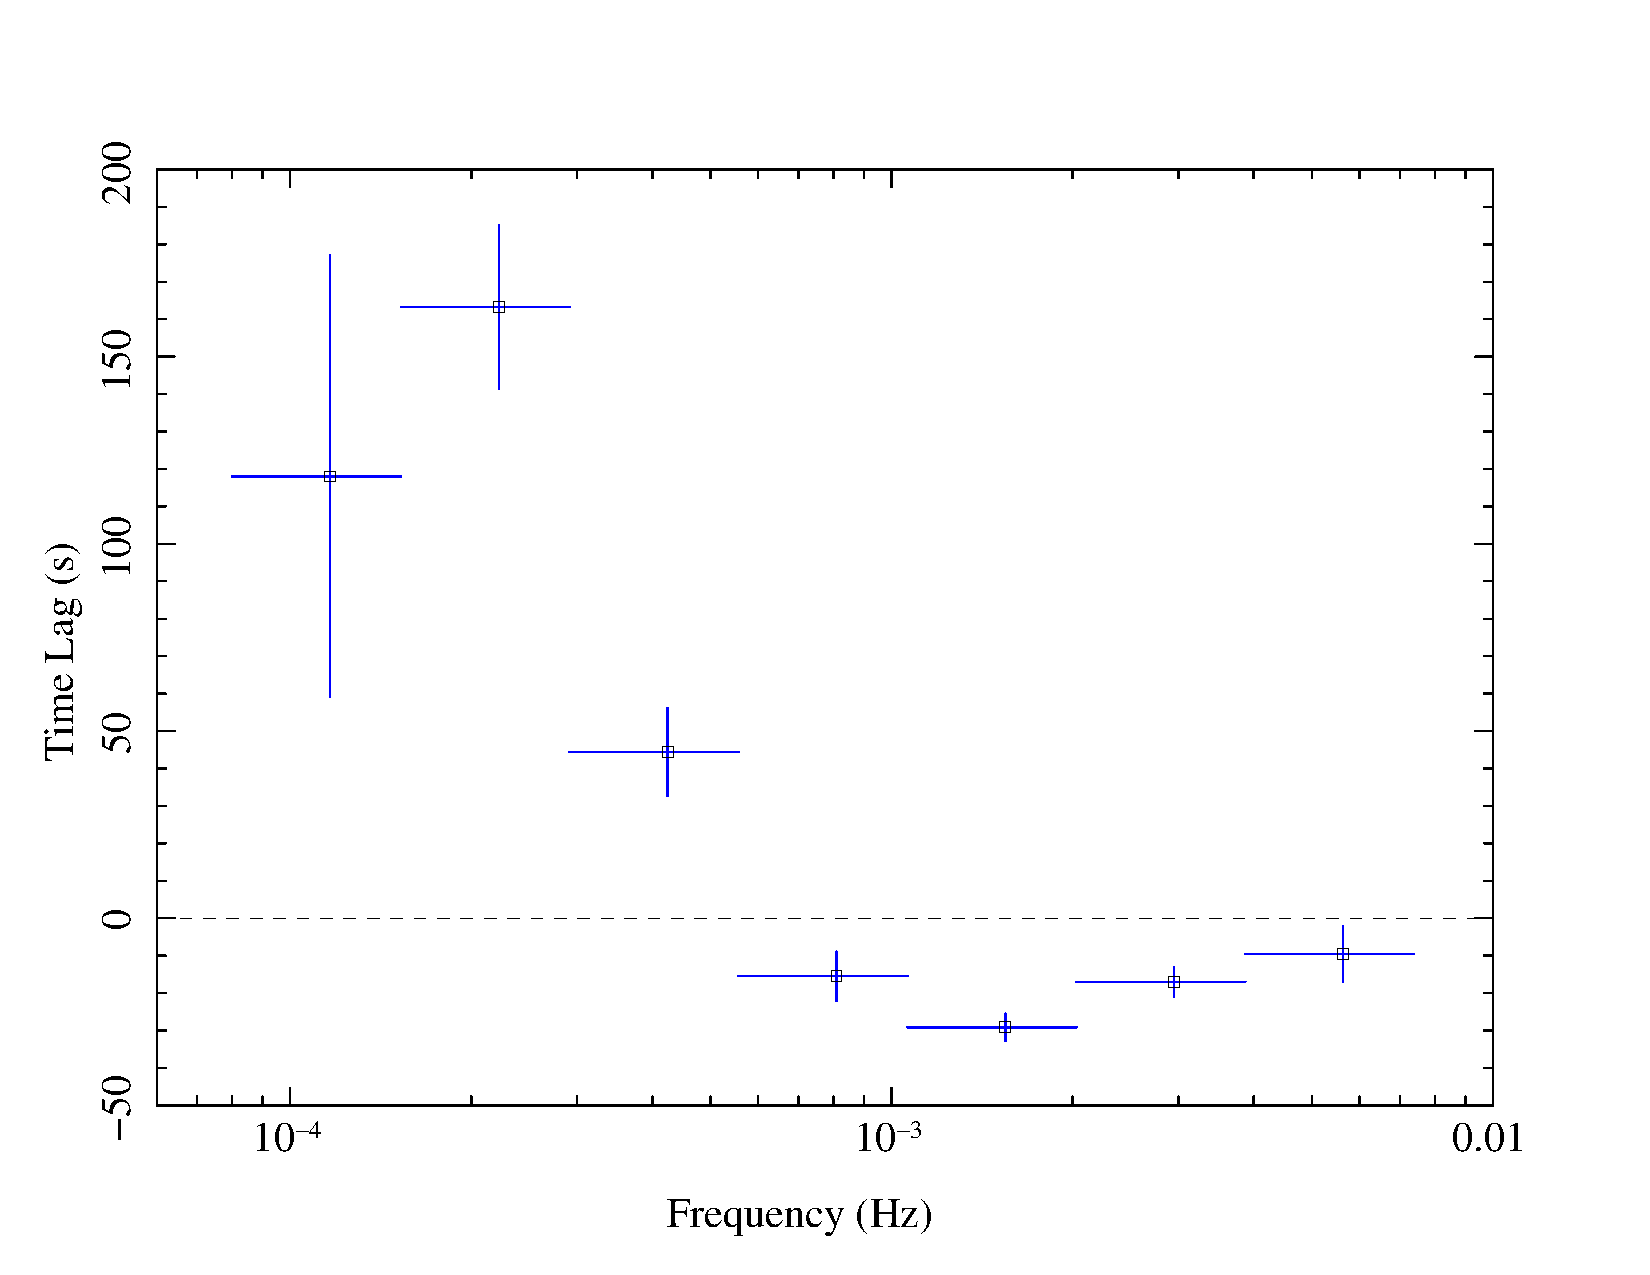
\includegraphics[scale=.25]{1H0707-495_lagfreq_fullycomb.pdf}}\\
Combined Lag-frequency from 15 XMM-Netwon observations between 2000-2011 showing a lag of $\sim30$s at 1.65 $\times 10^{-3}$ Hz.
\end{figure}
\end{frame}


\begin{frame}
\frametitle{Lag-frequency}
\begin{figure}\centering
\colorbox{white}{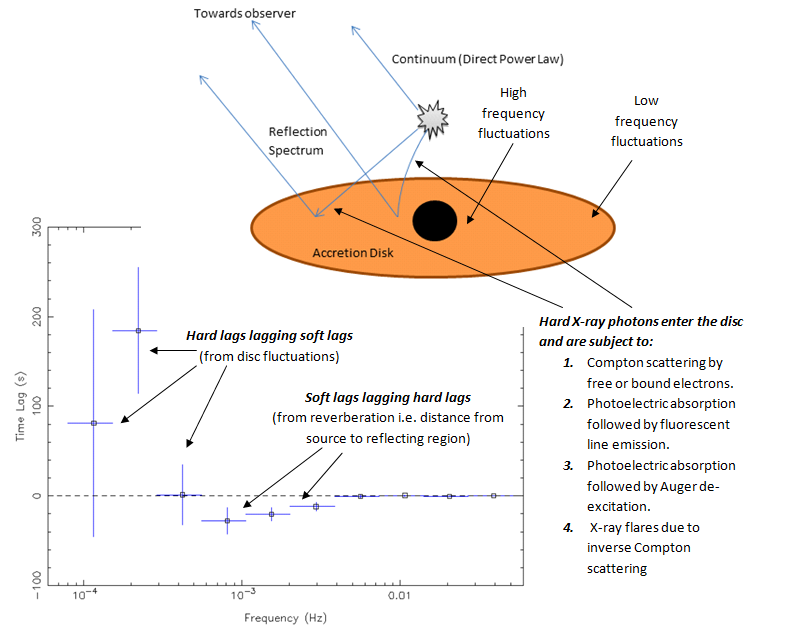
\includegraphics[scale=.45]{lags_explained.png}}\\
\end{figure}
\end{frame}

\begin{frame}
\frametitle{Soft Lag - Mass scaling relationship}
\begin{figure}\centering
\colorbox{white}{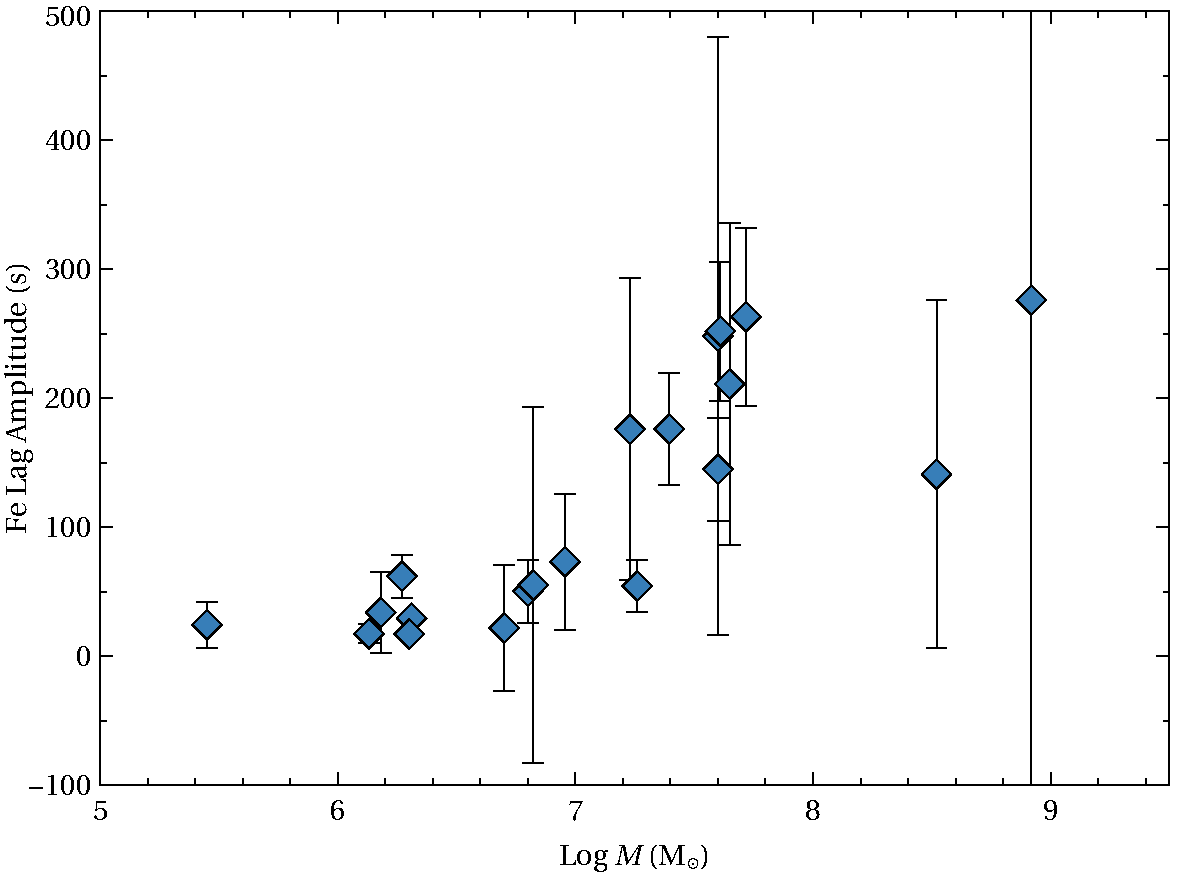
\includegraphics[scale=.40]{Fe_Lag_V_BHmass.pdf}}\\
Soft lags (typically $\sim 0.07 - 4 \times 10^{-4}$ Hz) have been discovered to scale with black hole mass (DeMarco + 2013).
\end{figure}
\end{frame}

\begin{frame}
\frametitle{Fitting ECM to 1H0707-495}
\begin{figure}\centering
\colorbox{white}{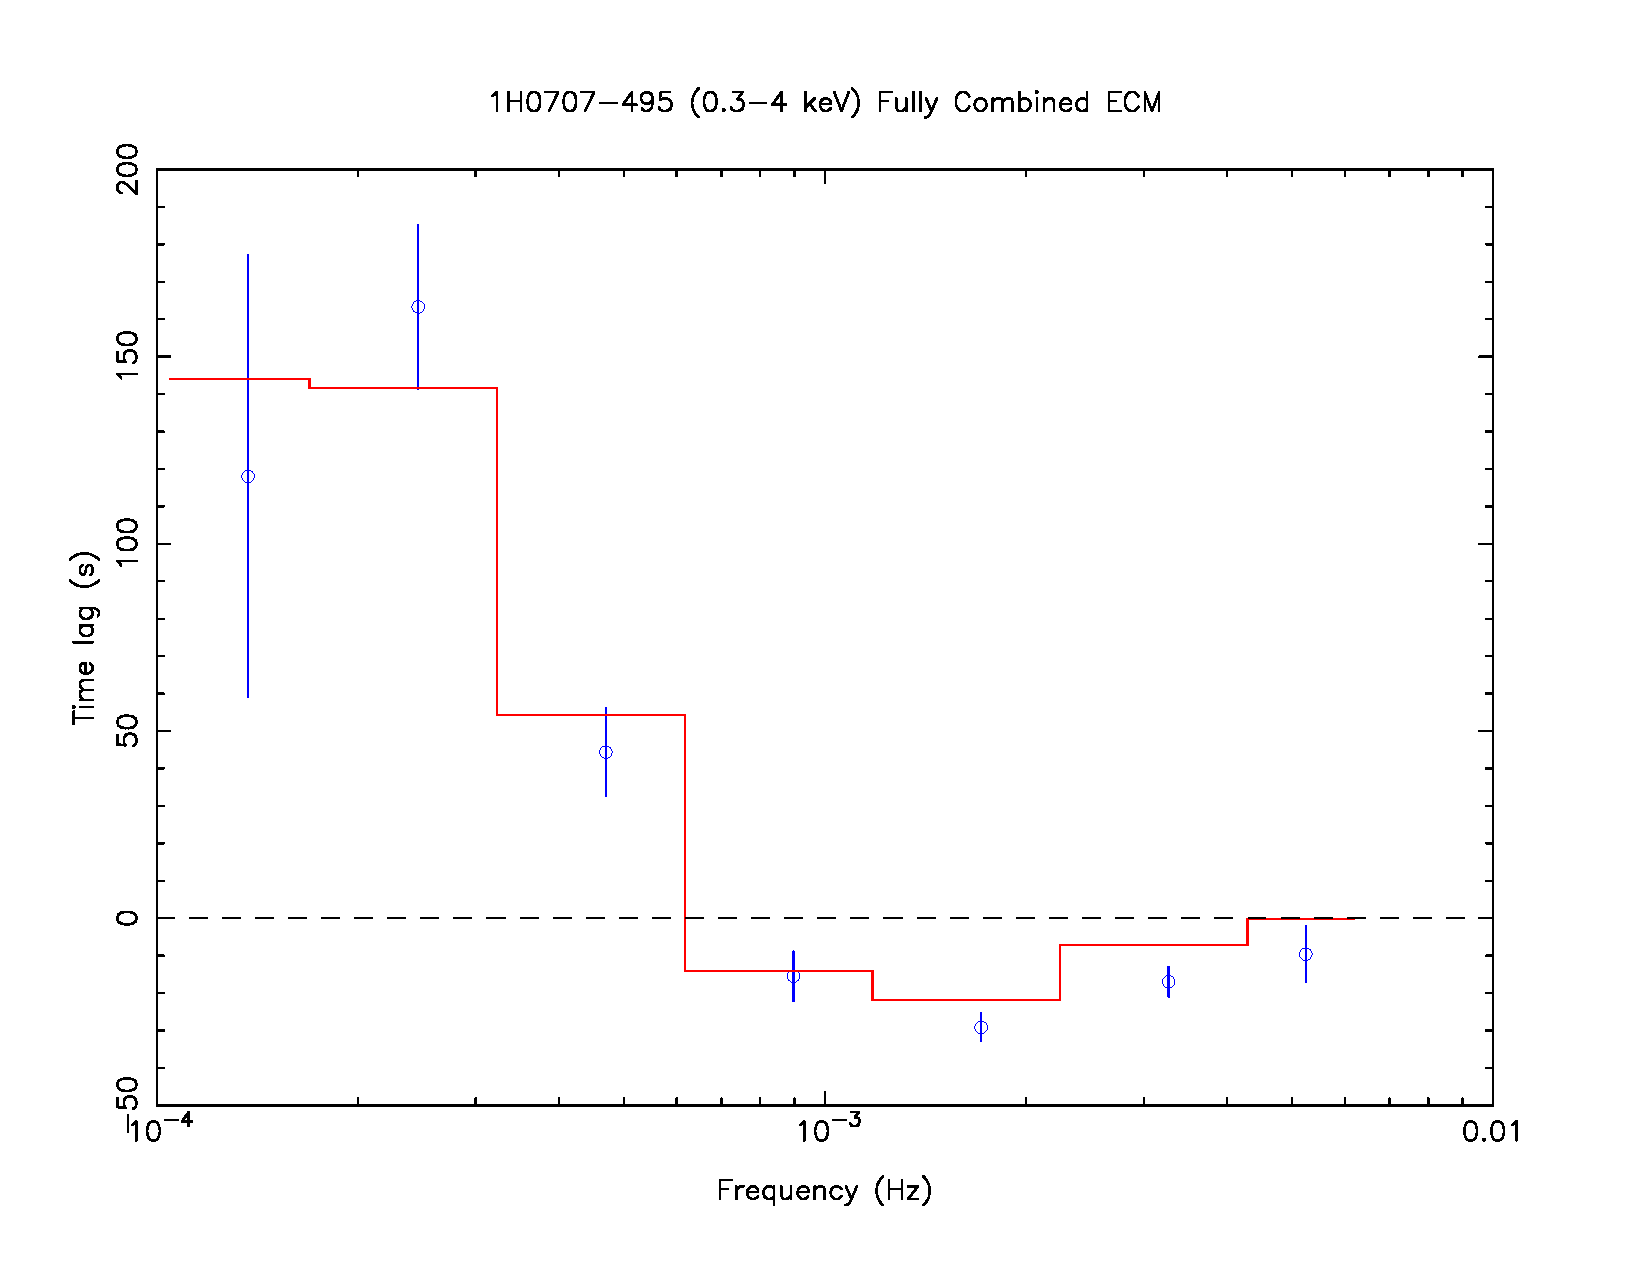
\includegraphics[scale=.25]{1H0707-495_fullycombECM.pdf}}\\
\begin{columns}
\column{0.15\textwidth}
\column{0.25\textwidth}
\begin{itemize}
    \item $h_1 = 2 r_g$
    \item $h_2 = 3 r_g$
\end{itemize}
\column{0.25\textwidth}
\begin{itemize}
    \item $t_\text{shift} = 74 t_g$
    \item $\chi^2 =  13.9$
\end{itemize}
\column{0.15\textwidth}
\end{columns}
\end{figure}
\end{frame}



\begin{frame}
\frametitle{The AGN Spectrum} \centering 
{
\begin{figure}
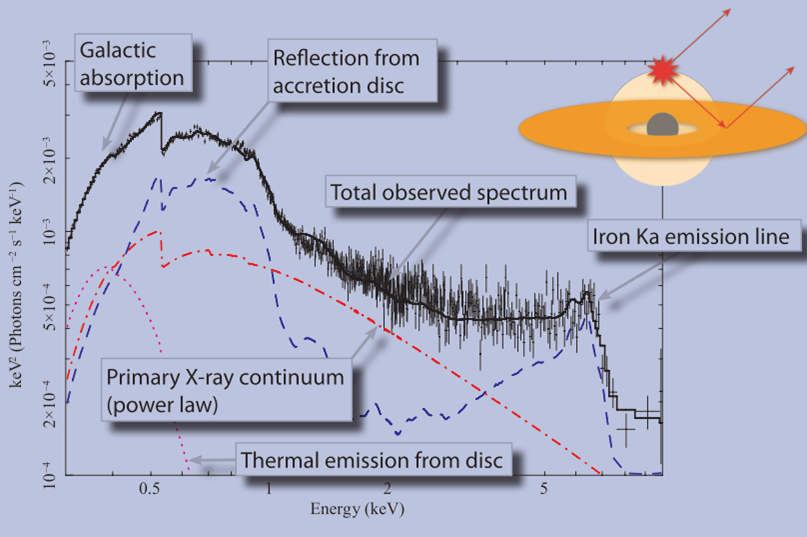
\includegraphics[scale=0.5]{AGN_spectra.png}\\
\caption{AGN IRAS13224-3809 Spectra (Wilkins, 2013)}
\end{figure}
}
\end{frame}


\begin{frame}
\frametitle{Improvement strategies}
\begin{itemize}
    \item Original fits were done with some basic assumptions of ionisation state, reflection fraction and system inclination\pause
    \item ECM model may demand greater scrutiny of individual AGN environmental parameters\pause
    \item Detailed analysis is key but AGN are highly variable- investigate different states of spectral variability (i.e. similar groups of flux seen from multiple observations)
\end{itemize}
\end{frame}

\begin{frame}
\frametitle{1H0707-495 Unfolded spectra 2000--2015}
\begin{figure}\centering
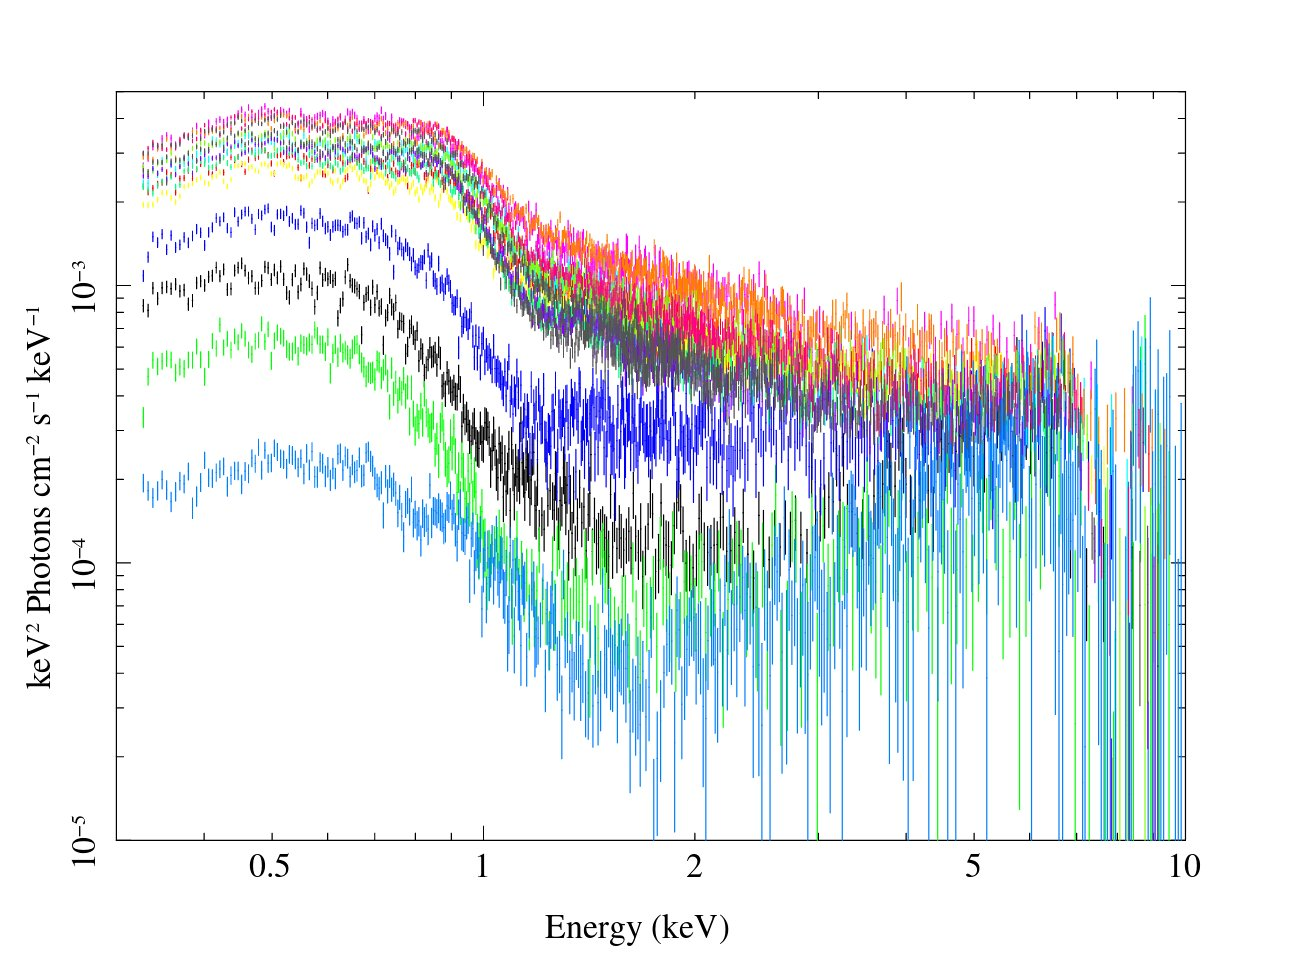
\includegraphics[scale=.25]{1H0707-495_Unfolded_Spectra.jpeg}
\end{figure}
% See \url{}
\end{frame}

\begin{frame}
\frametitle{1H0707-495 Unfolded spectra (2000-2015)}
\begin{figure}\centering
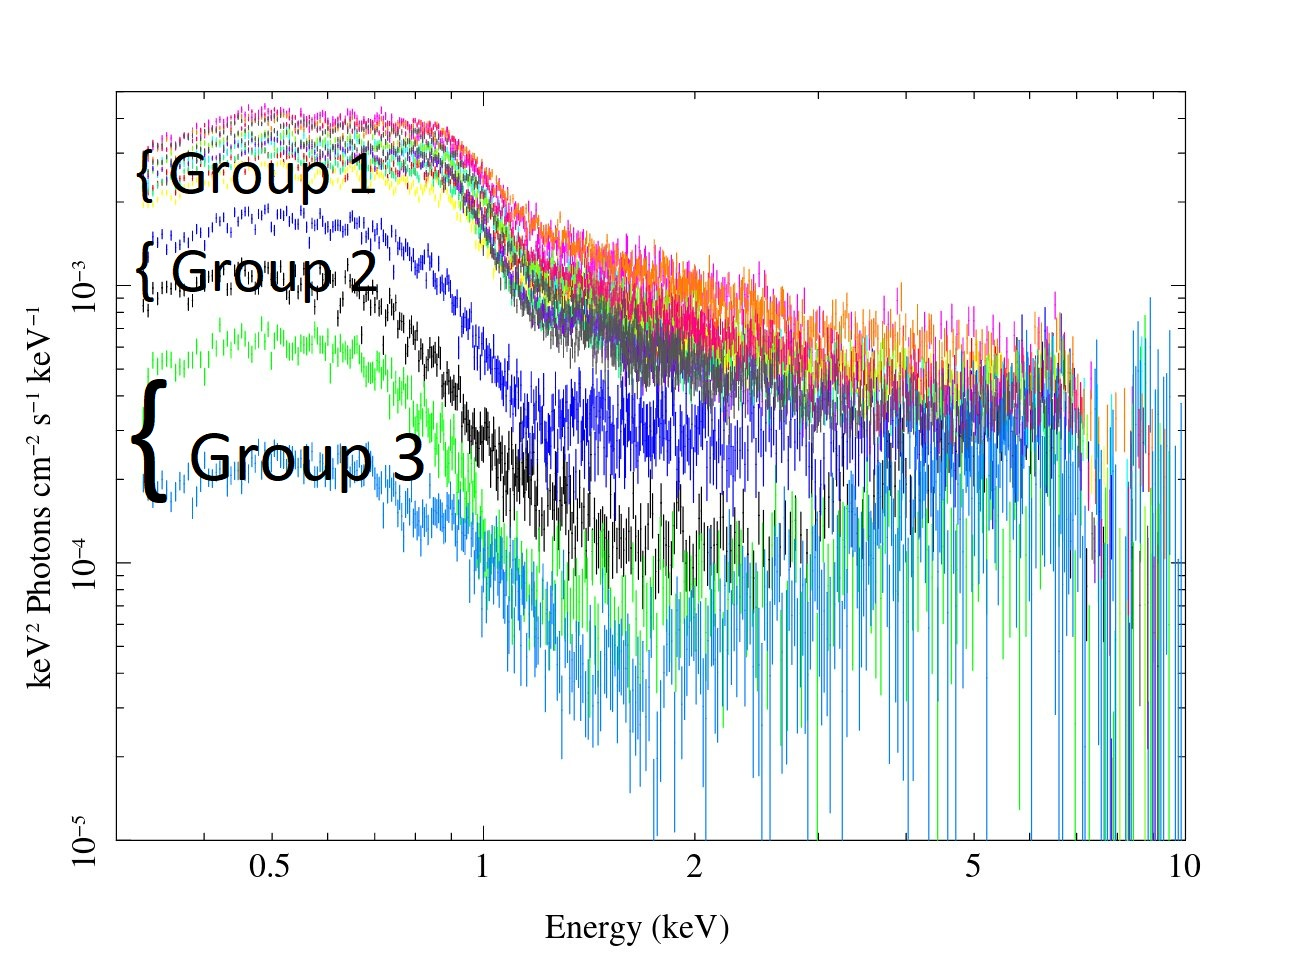
\includegraphics[scale=.25]{1H0707-495_Unfolded_Spectra_Grps.jpeg}
\end{figure}
\end{frame}

\begin{frame}
\frametitle{1H0707-495 Group 2 Spectra (Relxill*zpcfabs)}
\begin{figure}\centering
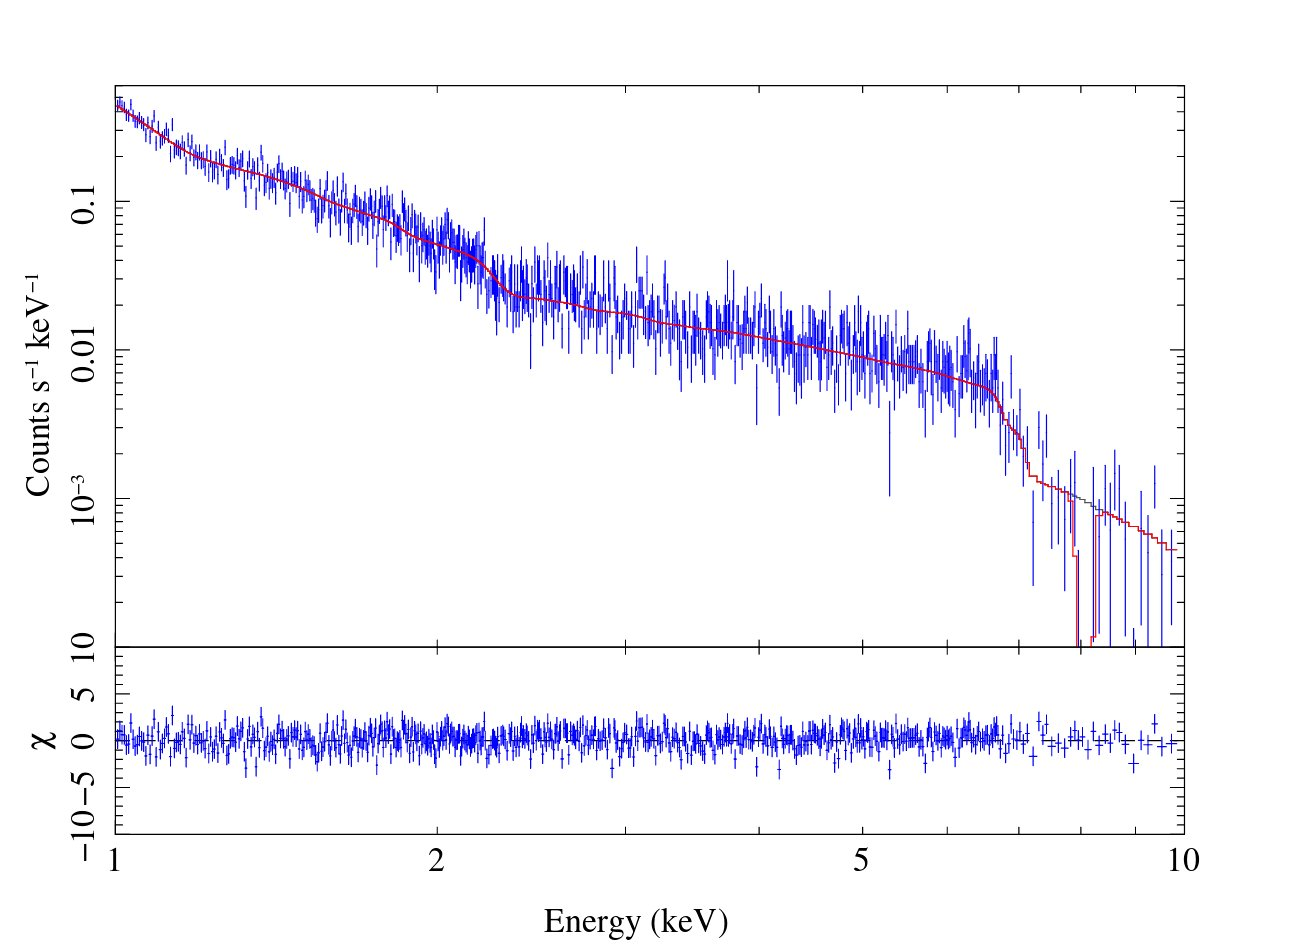
\includegraphics[scale=.25]{1H0707-495_Grp2_Spectra.jpeg}
\end{figure}
\end{frame}

\begin{frame}
\frametitle{1H0707-495 Group 2 Spectra (Relxill*zpcfabs)}
\centering
nH = $6.99^{+1.52}_{-1.35} \times 10^{22}$ cm$^{-2}$\\ \vspace{0.2cm}
CvrFract $ = 0.71^{+0.07}_{-0.20}$\\ \vspace{0.2cm}
$\Gamma = 2.93^{+0.07}_{-0.30}$\\ \vspace{0.2cm}
$a = 0.998^{f}$ \textit{(fixed)}\\ \vspace{0.2cm}
$z = 0.0411^{f}$ \textit{(fixed)}\\ \vspace{0.2cm}
$i = 71.17^{+6.59}_{-5.57}$ \textit{(known} $i = 57.5^\circ)$\\\vspace{0.2cm}
$Log\xi = 1.93^{+0.38}_{-0.55}$\\ \vspace{0.2cm}
$A_{FE}  = 0.50^{+0.00}_{-0.00}$\\ \vspace{0.2cm}
$R_f = 10.00^{+0.00}_{-1.30}$\\ \vspace{0.2cm}
$\chi^2 = 0.99$\\
\end{frame}

\begin{frame}
\frametitle{Mrk335 Unfolded Spectra (2006-2009)}
\begin{figure}\centering
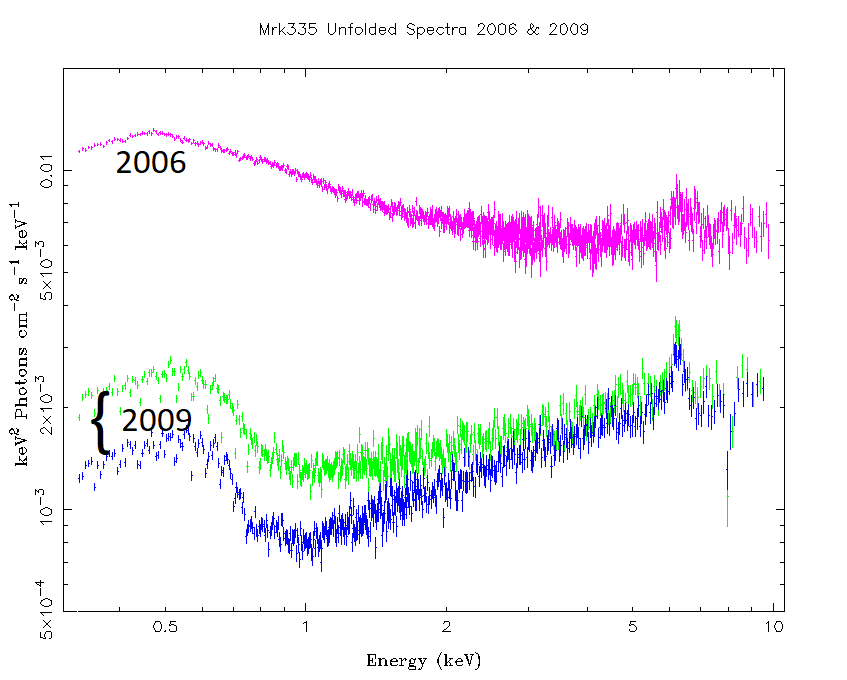
\includegraphics[scale=.40]{Mrk335_specall.png}
\end{figure}
\end{frame}

\begin{frame}
\frametitle{Mrk335 Folded Spectra 2006 (relxill*wabs)}
\begin{figure}\centering
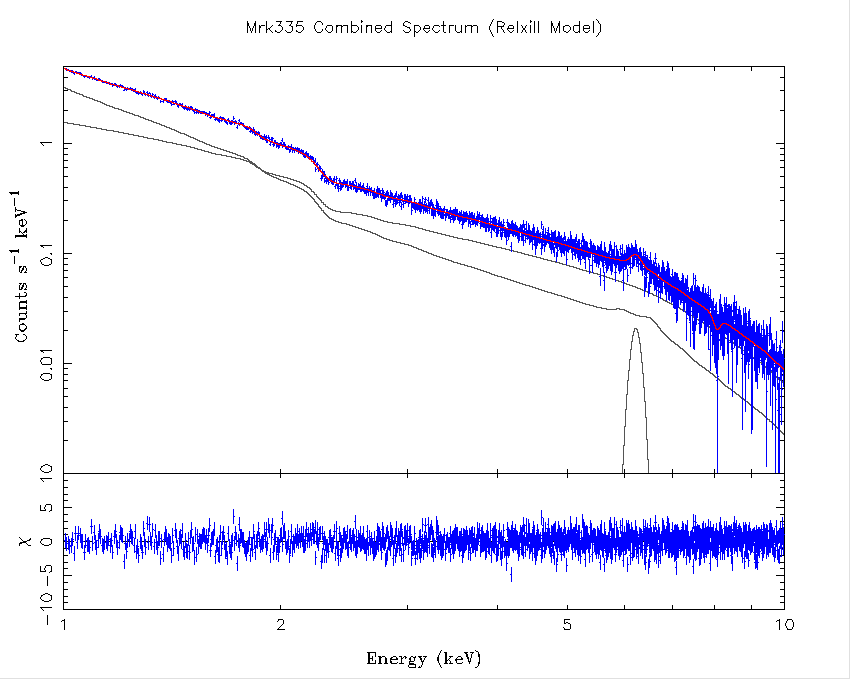
\includegraphics[scale=.40]{Mrk335_comb.png}
\end{figure}
\end{frame}


\begin{frame}
\frametitle{Mrk335 Folded Spectra 2006 (relxill*wabs)}
\begin{figure}\centering
\includegraphics[scale=.40]{Mrk335_2006.png}
\end{figure}
\end{frame}

\begin{frame}
\frametitle{Mrk335 Folded Spectra 2009 (relxill*wabs)}
\begin{figure}\centering
\includegraphics[scale=.40]{Mrk335_2009.png}
\end{figure}
\end{frame}

\begin{frame}
\frametitle{Mrk335 - All Spectra (relxill*wabs)}
\begin{table}
    \begin{tabular}{lrrr}\vspace{0.2cm}
        Parameter & Combined & 2006 & 2009
        \\ \hline \\ 
        \texttt{wabs} & $0.02^{+0.00}_{-0.02}$  & $0.00^{+0.06}_{-0.00}$ & $0.37^{+0.21}_{-0.27}$ \\ [1ex] 
        $\Gamma$ & $2.82^{+0.28}_{-0.20}$ & $2.33^{+0.06}_{-0.09}$ & $1.75^{+0.23}_{-0.12}$\\ [1ex] 
        $a$ &  $0.998^{f}$ &  $0.998^{f}$ &  $0.998^{f}$ \\ [1ex] 
        $z$ &  $0.0258^{f}$ &  $0.0258^{f}$ &  $0.0258^{f}$ \\ [1ex] 
        $i$ &  $69.62^{+8.97}_{-26.89}$ &  $44.36^{+2.48}_{-1.50}$ &  $32.38^{+8.79}_{-27.38}$ \\[1ex] 
        $Log\xi$ &  $0.82^{+0.25}_{-0.39}$ &  $0.73^{+0.27}_{-0.32}$ &  $0.10^{+3.13}_{-0.10}$\\ [1ex] 
        $A_{FE}$ &  $0.78^{+1.47}_{-0.23}$ &  $0.50^{+0.03}_{-0.00}$ &  $3.70^{+6.30}_{-2.50}$\\ [1ex] 
        $R_f$ & $10.00^{+0.00}_{-4.38}$ & $2.74^{+0.86}_{-0.72}$ & $1.13^{+4.64}_{-0.76}$\\ [1ex] \hline  
        $\chi^2$ & $1.35$ & $1.09$ & $1.13$\\ \hline  
    \end{tabular}
\end{table}
$f$ = fixed parameter
\end{frame}

\begin{frame}
\frametitle{Spectral analysis}
\begin{itemize}
    \item Reflection \& Absorption models required \pause
    \item Literature explored for individual AGN findings \pause
    \item General consistency used:\\
    \texttt{wabs*(powerlaw+relxill+diskbb)} 
    \texttt{zpcfabs*(powerlaw+relxill+diskbb)}\pause
    \item General agreement with previous literature findings and some new observations presented\pause
    \item Full \textit{working} Logbook online:
    \url{http://www.star.bris.ac.uk/steff/phd_ecm_logbook.html}\p
    \end{itemize}
\end{frame}

\begin{frame}
\frametitle{Spectral Grouping comparison}
\begin{figure}\centering
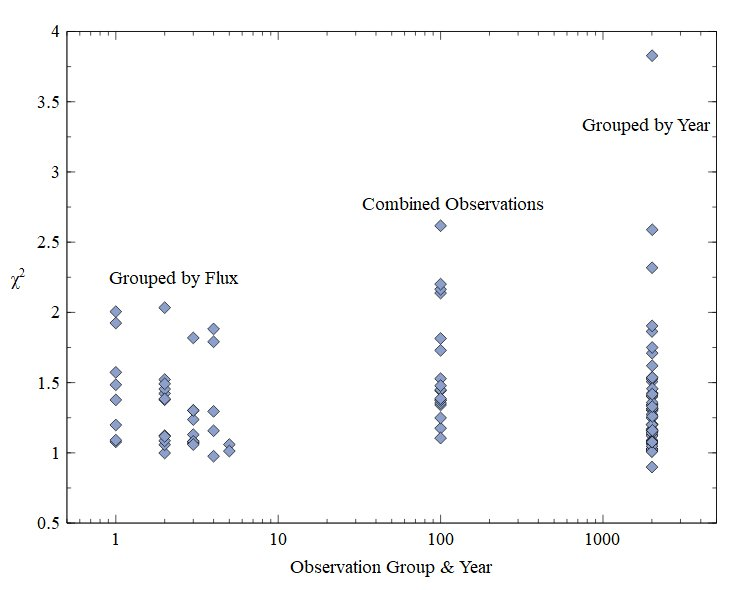
\includegraphics[scale=.5]{Spectral_fits_chi.jpg}
\end{figure}
\end{frame}
\begin{frame} <presentation:0>
\frametitle{Reflection Fraction}
Assuming a stationary isotropic X-ray source in lamp post geometry, the reflection fraction $\texttt{R}_f$ is defined as the ratio between the reflected and direct radiation.\pause
\begin{equation}
{
\texttt{R}_f = \frac{f_{\texttt{AD}}}{f_{\texttt{INF}}} = \frac{\texttt{cos}~\delta_{\texttt{in}} - \texttt{cos}~ \delta_{\texttt{out}}}{1 + \texttt{cos}~\delta_{\texttt{out}}}
}
\end{equation}

$f_{AD}$ and $f_{INF}$ are the fraction of the photons hitting the accretion disc or escaping to infinity respectively \pause\\
\vspace{0.2cm}
$\delta_{in}$ and $\delta_{out}$ are the angles under which photons hit the inner and outer edge of the disc respectively.\\
\vspace{0.2cm}
(Fukumura \& Kazanas 2007 ApJ 664, 14)
\end{frame}

\begin{frame} <presentation:0>
\frametitle{Reflection Fraction}
\begin{itemize}
\item In a previous study, (Dauser+2014) showed that high reflection fractions $\gtrsim 2$ are only possible for rapidly rotating black holes. \pause
\item This suggests that a high spin value will produce the strongest relativistic reflection. \pause
\item The \texttt{Relxill} model contains parameters describing dynamic features an accretion disc ranging from the marginally stable radius $R_\text{in} = 1.24 r_g$ to $R_\text{out} = 60 r_g$.\pause
\item \texttt{Relxill} includes full relativistic light bending effects that have been suggested to lead to the appearance of a warped disc.
\end{itemize} \end{frame}


\begin{frame}
\frametitle{Summary of previous results}
\begin{itemize} 
    \item Fixing the $M_{BH}$ to the known value and the $R_f$  to $\sim 0.2$ reveal $h_2$ source heights move through 3, 6 and 11$r_g$ during 2007, 2008 and 2010 respectively.\pause
    \item Statistically poor fits! - This study will improve \pause
    \item however.....
    \end{itemize}
\end{frame}

\begin{frame}
\frametitle{Similar flaring phenomenon seen in Mrk335}
\begin{figure}
\colorbox{white}{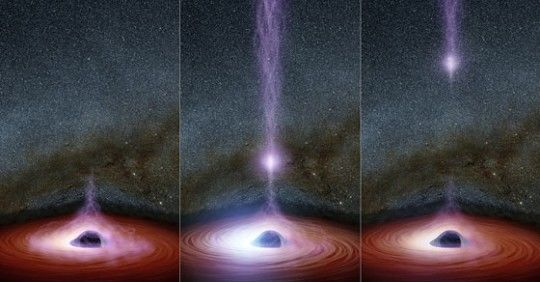
\includegraphics[scale=.35]{mrk335_jets.jpg}}\\
{\footnotesize  Wilkins et al (2015) reported a similar `flaring' phenomenon from \textit{Swift} and \textit{NuSTAR} observations of Mrk335. The X-ray spectrum was well described by the relativistically blurred reflection of the continuum from the accretion disc whose emissivity profile suggests that it is illuminated by a compact X-ray source, extending at most 5.2 $r_g$ over the disc and a very low reflection fraction of 0.41.}
\end{figure}
\end{frame}

\begin{frame}
\frametitle{Current Project Aims}
\begin{itemize}
    \item Produce spectral fits and ECM modelling for 20 AGN and publish findings (currently in prep)\pause
    \item Produce software to automate this pipeline and develop the Extended Corona Model for use by wider scientific community
    \end{itemize}
    \end{frame}

\begin{frame}
\frametitle{Summary}
\begin{itemize}
    \item The spectral variations of all AGN have been explored further and grouped into similar states in addition to the fully combined spectra and by the year of observation - vairiability is clearly apparent!
    \item All AGN spectra have been fitted (Combined/Year/Group) to reflection modelling, this includes absorption where deemed necessary \pause
    \item AGN parameters have been calculated and are ready to feed the ECM model `flavours'\pause
    \item Next - Refit ECM and explore the results\pause
    \item Finally - Automate pipeline and produce model 
    \end{itemize}
\end{frame}

\begin{frame}
\frametitle{Modelling available online}
All analysis is being documented online for easy collaboration\\
\begin{itemize}
    \item \url{http://www.star.bris.ac.uk/steff/phd_ecm_logbook.html} 
\end{itemize}
\end{frame}

\begin{frame}
\frametitle{Relativistic Accretion Disc} \centering 
{
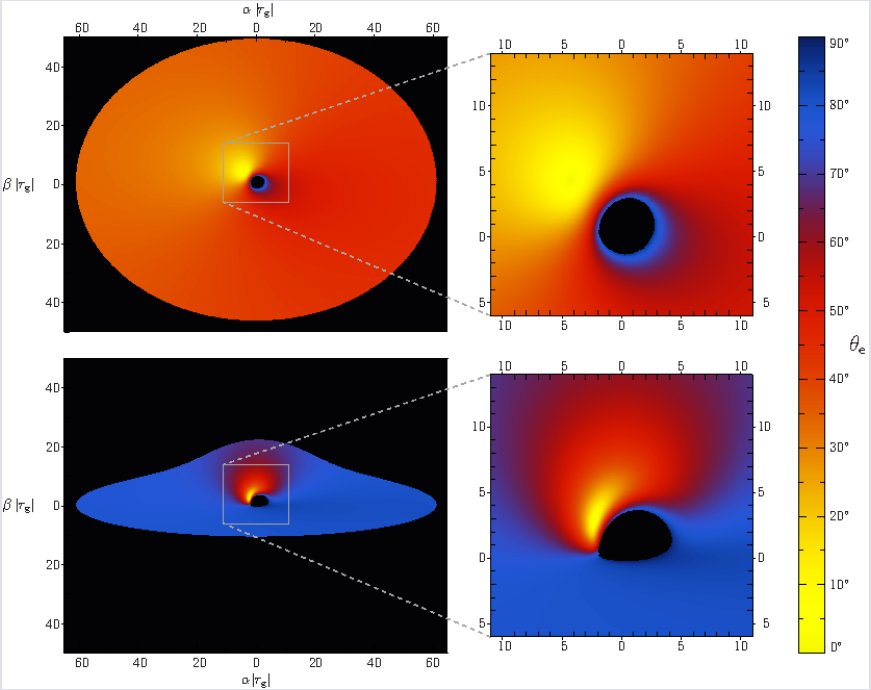
\includegraphics[scale=0.35]{relxill_rays.png}\\
\caption{Accretion disc viewed at angles $40^\circ$ (upper) and $80^\circ$ (lower). Angle $\theta_e$ can yield any value close to the black hole. Sky coordinates $\alpha$ and $\beta$ are perpendicular to the line of sight and the colour scale shows the energy shift of the photons - profile shows stronger variations closer to the centre (Dauser et al. 2010)}
}
\end{frame}


\begin{frame}
  \frametitle{References}

\begin{columns}
\column{0.5\textwidth}
{\footnotesize  
\begin{itemize} 
  \item{Balbus \& Hawley (1991) ApJ 376, 214}
  \item{Chainakun \& Young (2017) MNRAS, 465, 3965}
  \item{Dauser et al (2014) MNRAS, Letters, 444, L100} 
  \item{Fabian \& Vaughan (2003) MNRAS,340,L28}
  \item{Fukumura \& Kazanas (2007) ApJ 664, 14}
  \item{Miller \& Turner (2011) Proceedings of Science, arXiv:1106.3648v1}
\end{itemize}
}
\column{0.5\textwidth}
{\footnotesize
\begin{itemize}
    \item{Miniutti et al (2003) MNRAS, 344, L22-L26}
  \item{Miniutti \& Fabian (2004) MNRAS, 349, 1435}
  \item{Nowak et al (1999) ApJ 510, 874}
  \item{Tanaka et al (1995) Nature, 375, 659}
  \item{Uttley et al (2014) A\&A 22, 1}
  \item{Wilkins (2013), 2013HEAD...1310813W}
  \item{Wilkins et al (2015) MNRAS, 454, 4440-4451}
\end{itemize}
}
\end{columns}
\end{frame}

\begin{frame}
\frametitle{Questions}
\begin{figure}\centering
\colorbox{white}{
\includegraphics[scale=.4]{Questions1.png}}\\
\end{figure}
\end{frame}


\begin{frame}<presentation:0>
[t]{Title of frame}
    \begin{columns}[T,onlytextwidth]
        \begin{column}{.4\textwidth}
            \begin{minipage}{\textwidth}
                \begin{figure}
                    \includegraphics[width=\textwidth]{example-image}
                \end{figure}
                \footnotetext{Figure left top}
            \end{minipage}  
            \begin{onlyenv}<3>
                \begin{minipage}{\textwidth}
                    \begin{figure}
                        \includegraphics[width=\textwidth]{example-image}
                    \end{figure}
                \footnotetext{Figure left bottom}
                \end{minipage}
            \end{onlyenv}
        \end{column}
        \begin{column}{.4\textwidth}
            \begin{onlyenv}<2->
                \begin{minipage}{\textwidth}
                    \begin{figure}
                        \includegraphics[width=\textwidth, height=.77\textheight]{example-image}
                    \end{figure}
                    \footnotetext{Figure right}
                \end{minipage}
            \end{onlyenv}
        \end{column}
    \end{columns}
\end{frame}
\end{document}

\begin{frame}<presentation:0>
\frametitle{There Is No Largest Prime Number}
%\framesubtitle{The proof uses \textit{reductio ad absurdum}.}
\begin{theorem}
There is no largest prime number.
\end{theorem}
\begin{proof}
\begin{enumerate}
\item<1-| alert@1> Suppose $p$ were the largest prime number.
\item<2-> Let $q$ be the product of the first $p$ numbers.
\item<3-> Then $q+1$ is not divisible by any of them.
\item<1-> But $q + 1$ is greater than $1$, thus divisible by some prime
number not in the first $p$ numbers.\qedhere
\end{enumerate}
\end{proof}
\end{frame}

\begin{frame}<presentation:0>
{Frame 1}
  \begin{multicols}{2}
    \begin{minipage}[b][20ex][t]{\linewidth}
      Section 1
      \begin{itemize}
        \item<1-> Item 1
        \item<2-> Item 2
        \item<3-> Item 3
      \end{itemize}
    \end{minipage}

    \begin{minipage}[b][20ex][t]{\linewidth}
      Section 2

      \only<1>{
        Content 1 in section 2
      }
      \only<2>{
        Content 2 in section 2
      }
      \only<3>{
        Content 3 in section 2
      }
    \end{minipage}

    \begin{minipage}[b][40ex][t]{\linewidth}
      Section 3

      \only<1>{
        Content 1 in section 3
      }
      \only<2>{
        Content 2 in section 3
      }
      \only<3>{
        Content 3 in section 3
      }
    \end{minipage}
  \end{multicols}
\end{frame}